\section{Modeling approach}
\label{sec:prelims}

We extend the setting of \textcite{ingrosso2022data},
a minimal example of a neural network that learns localized receptive fields 
from idealized naturalistic data.
We analyze the dynamics of learning in this setting in \cref{sec:theory}
and validate our analytical model with simulations in \cref{sec:experiments}.

\subsection{Neural network architecture and learning algorithm}
\label{sec:model}

We consider a two-layer feedforward neural network with nonlinear activation and scalar output.
While simple, this architecture is highly expressive, capable of approximating arbitrary 
integrable univariate functions with appropriate scaling~\parencite{barron1993universal, pinkus1999approximation},
and exhibits rich feature learning dynamics that underlie the performance of models at scale~\parencite{woodworth2020kernel},
making this architecture the ongoing subject of theoretical neural network analyses~\parencite{mei2018mean, goldt2019dynamics, veiga2022phase}.
We denote a two-layer network with $N$-dimensional input, $M$ hidden units, and one-dimensional scalar output as
\newcounter{modelenumi}
\begin{model}{\textbf{Model 1} (\emph{many-neuron architecture}).}{}
\begin{enumerate}[series=modelenumi]
  \item \label{item:many-neuron-model} 
    \makebox[\linewidth - 2.5em]{
      $\hat{y}(\mathbf{x}) = b^{(2)} + \sum_{m=1}^M w_m^{(2)} 
      \sigma\left(b_m^{(1)} + \langle \mathbf{w}_m^{(1)}, \mathbf{x} \rangle \right)$
    }
\end{enumerate}
\end{model}
where $\sigma : \R \to \R$ is a pointwise nonlinearity such as the rectified linear unit (ReLU) or sigmoid function,
$\mathbf{w}_m^{(1)} \in \R^N$ and $w_m^{(2)} \in \R$ are learnable weights, 
$b_m^{(1)}, b^{(2)} \in \R$ are learnable bias terms, and
$\langle \cdot, \cdot \rangle$ denotes the standard Euclidean inner (dot) product on $\R^N$.
When the second-layer parameters are fixed, this model is known as a \emph{soft-committee machine}~\parencite[SCM;][]{saad1995line},
which~\parencite{ingrosso2022data} notes learns less noisy receptive fields but exhibits similar localization behavior.
The many-neuron architecture in \labelcref{item:many-neuron-model} is the focus of our \textbf{simulations}~(\cref{sec:experiments}), but the dynamics of this model 
are too complex to analyze directly, even for the idealized naturalistic data model considered here.
In order to derive \textbf{analytical} results~(\cref{sec:theory}), we consider the simplest neural network exhibiting the desired localization phenomenon, a single hidden neuron without bias and with rectified linear unit activation, written as
\begin{model}{\textbf{Model 2} (\emph{single-neuron architecture}).}{}
\begin{enumerate}[resume*=modelenumi]
  \item \label{item:single-neuron-model} 
    \makebox[\linewidth - 2.5em]{
      $\hat{y}(\mathbf{x}) = 
      \operatorname{ReLU}\left(\langle \mathbf{w}, \mathbf{x} \rangle \right)$
    }
\end{enumerate}
\end{model}
where $\operatorname{ReLU}(x) = \max(x,0)$, applied pointwise to vectorial input.
As \textcite{ingrosso2022data} demonstrate, the localized receptive fields learned by the 
many- and single-neuron models defined in \labelcref{item:many-neuron-model,item:single-neuron-model} are qualitatively similar up to spatial translation, 
which permits us to generalize insights from analyzing the learning dynamics of the single-neuron~\labelcref{item:single-neuron-model} to the many-neuron~\labelcref{item:many-neuron-model}.
For simulations, we initialize the weights and biases
as independent draws from an isotropic Gaussian distribution with scaled variance,
and train with batch gradient descent with a fixed learning rate on the mean-squared error
(MSE) evaluated on input-output pairs from the task; see \cref{sec:task} for task sampling procedures.

\subsection{Stimulus properties}
\label{sec:input}

The data model of \textcite{ingrosso2022data} 
can be shown to satisfy three conditions that enable the analysis we give in \cref{sec:theory}.
We consider several other data models that share the below properties but differ in generative mechanism
in order to probe the effect of these properties on localization.
In particular, we consider data $\mathbf{X}$ sampled from distributions $p$ on $\R^N$ satisfying the following:
\newcounter{propenumi}
\begin{stimulus}{\textbf{Stimulus properties 1--3} (\emph{idealization of natural images}).}{}
\begin{enumerate}[series=propenumi]
  \item \label{item:weak-dependence} (Positional) weak dependence: for any fixed $\rho \in (0,1)$, as $N \to \infty$,
    $$\alpha(N) \triangleq \sup_{A \subseteq \R, B \subseteq \R^{(1-\rho) N}} |\PR(X_1 \in A, X_{> \rho N} \in B) - \PR(X_1 \in A) \PR(X_{> \rho N} \in B)| \to 0~,$$
  \item \label{item:translation-invariance} Translation invariance: $p(\mathbf{X} = \mathbf{x}) = p(\mathbf{X} = \mathcal{S} \mathbf{x})$ for all $\mathbf{x} \in \R^N$, where $\mathcal{S}$ is the circular shift operator, and
  \item \label{item:sign-symmetry} Sign symmetry: $p(\mathbf{X} = \mathbf{x}) = p(\mathbf{X} = -\mathbf{x})$ for all $\mathbf{x} \in \R^N$.
\end{enumerate}
\end{stimulus}
Properties~\labelcref{item:weak-dependence,item:translation-invariance}
are defining characteristics of natural image data~\parencite{hyvarinen2009natural}.
Property~\labelcref{item:sign-symmetry}
can also be seen to hold for natural images after centering
and is convenient analytically
because it implies that $\E[\mathbf{X}] = 0$.
Property~\labelcref{item:weak-dependence} assumes that $p$ is implicitly parameterized by $N$
in order to state that the statistical dependence between entries of $\mathbf{X}$ vanishes 
as their separation increases.\smash{\footnotemark}\footnotetext{
  The weak dependence condition in \labelcref{item:weak-dependence} is based on strong $\alpha$-mixing, a notion first introduced by \cite{rosenblatt1956central} 
  to obtain a generalization of the central limit theorem, which we employ later on.
  We choose $\alpha$-mixing because it is easy to interpret and verify,
  but alternative definitions of weak dependence \parencite[\eg][]{bardet2008dependent} can be substituted.
}

We denote the covariance of $\mathbf{X}$ by $\Sigma \triangleq \operatorname{Cov}[\mathbf{X}]$,
the square of principal-diagonal entries (the variance of each entry of $\mathbf{X}$) by $\sigma^2$, 
and the $i$-th row by $\sigma_i$.
Weak dependence (\labelcref{item:weak-dependence}) implies that entries far from the principal diagonal of $\Sigma$ will be 0, while translation-invariance (\labelcref{item:translation-invariance}) implies that $\Sigma$ is circulant (\ie entries along each diagonal are equal) and thus identifiable by a single row; see \cref{fig:task} (center).

\subsection{Lengthscale discrimination task}
\label{sec:task}

\textcite{ingrosso2022data} develop a minimal task for which localization emerges in a feedforward neural network: binary discrimination between inputs from two distributions that differ in the lengthscale of the correlations between their entries.
This lengthscale discrimination task can be seen as a pretext task for self-supervised learning~\parencite{kolesnikov2019revisiting,chen2020simple} of representations~\parencite[\cf~unsupervised:][]{olshausen1996emergence,bell1997independent}.
More precisely, we generate data $(\mathbf{X},Y)$ for supervised training according to
\begin{align} \label{eq:task}
    \mathbf{X} \mid Y = y \sim p(\mathbf{X};\Sigma_y)~,
\end{align}
where $p$ is to be defined, $\Sigma_y$ are distinct covariance matrices for each $y$, and we sample $Y$ uniformly among a set of increasing \emph{lengthscale correlation classes} $y \in \{0,1,\ldots\}$, which correspond to the strength of correlation between distant positions.
For instance, in the case of two classes ($y = 0, 1$), we take $\Sigma_0$ to be closer to $\sigma^2 \mathbb{I}_N$ than $\Sigma_1$, where $\mathbb{I}_N$ is the $N \times N$ identity matrix and $\sigma$ is a fixed value.
This construction isolates, via distinct covariance matrices per class, the second-order statistics, which we will see below enter into the learning dynamics separately from other properties of $p(\mathbf{X})$, including, most critically, the implied marginal distributions, $p(X_i)$.

\paragraph{\texttt{Ising}.}\hspace{-2pt}
The first distribution we consider is the one-dimensional Ising model.
It is of interest as a distribution that satisfies \labelcref{item:weak-dependence,item:translation-invariance,item:sign-symmetry} with marginals $p(X_i)$ with extreme support on $\{ \pm 1 \}$,
making it the distribution that promotes localization most strongly, as we will see in \cref{sec:theory}.
In the absence of an external field, the Ising distribution is
\begin{equation}
    p_\text{\texttt{Ising}}(\mathbf{X}=\mathbf{x})
    = p_\text{\texttt{Ising}}(X_1=x_1,\ldots,X_N=x_N) = e^{ -\sum_{i=1}^{N} J x_i x_{i+1} } / \mathcal{Z},
\end{equation}
where $J$ is a chosen pairwise interaction strength, $\mathcal{Z}$ is the normalizing constant, and we enforce a periodic boundary constraint via $x_{N+1} \equiv x_1$.
As $J$ increases, the lengthscale of the correlations in $\mathbf{X}$ also increases.
For simulations, we sample from $p_\texttt{Ising}$ using a Gibbs sampler~\parencite{geman1984stochastic}.
Discrimination tasks in the simulations in 
\cref{sec:experiments}
use $J_1=0.7$ (for $y=1$) and $J_0=0.3$ (for $y=0$).

\begin{wrapfigure}{l}{0.45\textwidth}
    \centering
    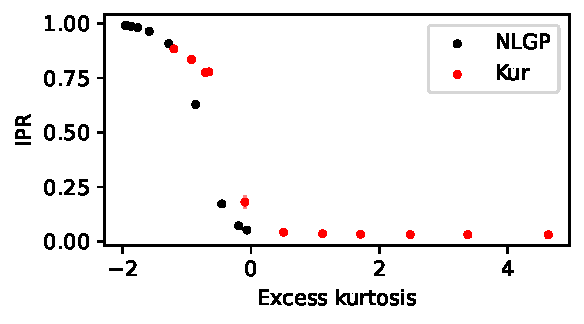
\includegraphics[width=170pt]{rebuttal-figures/replications/kurtosis_vs_ipr_40.pdf}
    \caption{
    IPR \vs excess kurtosis for $\texttt{NLGP}$ and $\texttt{Kur}$ data models, with mean and std.~dev.~across 30 re-initializations for the single-neuron model (\labelcref{item:single-neuron-model});
    error bars are small and may not be visible.
    }
    \label{fig:replications}
    \vspace{-14pt}
\end{wrapfigure}


\paragraph{\texttt{NLGP}$(g)$.}\hspace{-2pt}
We also consider the data model used in \textcite{ingrosso2022data}, the nonlinear Gaussian process (NLGP), which enables one to interpolate between distributions that do and do not yield localization via a single parameter, $g$.
A sample $\mathbf{X} \mid Y = y$ from the NLGP is constructed by first sampling a Gaussian $\mathbf{Z} \mid Y = y \sim \NN(0, \tilde{\Sigma}_y)$ and then transforming it via
\begin{equation} \label{eq:nlgp}
    X_i \triangleq \operatorname{erf}(g Z_i) / \mathcal{Z}(g) \qquad 1 \leq i \leq N,
\end{equation}
where $\operatorname{erf}$ is the Gauss error function, $\mathcal{Z}$ is a normalization constant to ensure that the variances of $X_i$ and $Z_i$ are the same, and $\tilde{\Sigma}_y$ is a covariance matrix for $\mathbf{Z}$, where we use $(\tilde{\Sigma}_y)_{ij} = \exp(-(i-j)^2/\xi^2)$ for a lengthscale parameter $\xi$ \cite{ingrosso2022data}. 
If $g \approx 0$ (where localization is \emph{not} observed), $g Z_i$ will tend to lie in the linear regime of $\operatorname{erf}$, so $Z_i$ will be untransformed, \ie $\mathbf{X}$ is Gaussian.
However, as $g \to \infty$ (where localization \emph{is} observed), $g Z_i$ will tend to saturate $\operatorname{erf}$, so $X_i$ will have support on $\{ \pm 1 \}$.

\paragraph{\texttt{Kur}$(k)$.}\hspace{-2pt}
The final family we consider is chosen to give us flexibility over the kurtosis $\kappa$ of the marginals $p(X_i)$.
In the Ising model, the \emph{excess} kurtosis ($\kappa - 3$) of the marginals is fixed at $-2$, while in $\texttt{NLGP}(g)$, it varies from $-2$ to $0$.
This family allows us to vary the excess kurtosis from negative through positive values.
We sample $\mathbf{X} \mid Y = y$ from this family via inverse transform sampling to vary the marginals while enforcing dependence via Gaussian copulas.
More concretely, we sample $\mathbf{Z} \mid Y = y \sim \NN(0, \tilde{\Sigma}_y)$ and then transform it via
\begin{equation}
    X_i \triangleq f^{-1}( \Phi( Z_i / \tilde{\sigma} )) / \mathcal{Z}, \qquad 1 \leq i \leq N, \label{eq:alg}
\end{equation}
where $\tilde{\sigma}$ is the standard deviation of $Z_i$, $\Phi$ is the standard Gaussian cumulative distribution function (CDF), $f$ is the CDF of the desired marginal distribution for $X_i$, and $\mathcal{Z}$ is a normalization constant, which we compute numerically.
We define $\tilde{\Sigma}_y$ as for $\texttt{NLGP}$.
We choose $f$ to be the generalized \emph{algebraic sigmoid} function (see \cref{sec:algebraic-sigmoid})
for $k > 0$ to make use of its tractable inverse, simplifying the procedure in \cref{eq:alg}.
We denote the corresponding distribution by $\texttt{Kur}(k)$.
Though we are able to continuously vary excess kurtosis, we lack an explicit form; however, numerical computation shows that for $k \lessapprox 5.8$, excess kurtosis is positive, while for $k \gtrapprox 5.9$, it is negative.
